\documentclass[english,]{IEEEtran}
\usepackage{lmodern}
\usepackage{amssymb,amsmath}
\usepackage{ifxetex,ifluatex}
\usepackage{fixltx2e} % provides \textsubscript
\ifnum 0\ifxetex 1\fi\ifluatex 1\fi=0 % if pdftex
  \usepackage[T1]{fontenc}
  \usepackage[utf8]{inputenc}
\else % if luatex or xelatex
  \ifxetex
    \usepackage{mathspec}
  \else
    \usepackage{fontspec}
  \fi
  \defaultfontfeatures{Ligatures=TeX,Scale=MatchLowercase}
\fi
% use upquote if available, for straight quotes in verbatim environments
\IfFileExists{upquote.sty}{\usepackage{upquote}}{}
% use microtype if available
\IfFileExists{microtype.sty}{%
\usepackage{microtype}
\UseMicrotypeSet[protrusion]{basicmath} % disable protrusion for tt fonts
}{}
\usepackage[unicode=true]{hyperref}
\hypersetup{
            pdftitle={A Survey of Techniques for Price Stabilisation of Cryptocurrencies},
            pdfkeywords={Stablecoin, Blockchain, Cryptocurrencies},
            pdfborder={0 0 0},
            breaklinks=true}
\urlstyle{same}  % don't use monospace font for urls
\ifnum 0\ifxetex 1\fi\ifluatex 1\fi=0 % if pdftex
  \usepackage[shorthands=off,main=english]{babel}
\else
  \usepackage{polyglossia}
  \setmainlanguage[]{english}
\fi
\usepackage{longtable,supertabular,booktabs}
% Fix footnotes in tables (requires footnote package)
\IfFileExists{footnote.sty}{\usepackage{footnote}\makesavenoteenv{long table}}{}
\usepackage{graphicx,grffile}
\makeatletter
\def\maxwidth{\ifdim\Gin@nat@width>\linewidth\linewidth\else\Gin@nat@width\fi}
\def\maxheight{\ifdim\Gin@nat@height>\textheight\textheight\else\Gin@nat@height\fi}
\makeatother
% Scale images if necessary, so that they will not overflow the page
% margins by default, and it is still possible to overwrite the defaults
% using explicit options in \includegraphics[width, height, ...]{}
\setkeys{Gin}{width=0.8\maxwidth,height=0.8\maxheight,keepaspectratio}
\IfFileExists{parskip.sty}{%
\usepackage{parskip}
}{% else
\setlength{\parindent}{0pt}
\setlength{\parskip}{6pt plus 2pt minus 1pt}
}
\setlength{\emergencystretch}{3em}  % prevent overfull lines
\providecommand{\tightlist}{%
  \setlength{\itemsep}{0pt}\setlength{\parskip}{0pt}}
\setcounter{secnumdepth}{5}
% Redefines (sub)paragraphs to behave more like sections
\ifx\paragraph\undefined\else
\let\oldparagraph\paragraph
\renewcommand{\paragraph}[1]{\oldparagraph{#1}\mbox{}}
\fi
\ifx\subparagraph\undefined\else
\let\oldsubparagraph\subparagraph
\renewcommand{\subparagraph}[1]{\oldsubparagraph{#1}\mbox{}}
\fi

% set default figure placement to htbp
\makeatletter
\def\fps@figure{htbp}
\makeatother

\makeatletter
\let\oldlt\longtable
\let\endoldlt\endlongtable
\def\longtable{\@ifnextchar[\longtable@i \longtable@ii}
\def\longtable@i[#1]{\begin{figure}[t]
\onecolumn
\begin{minipage}{0.5\textwidth}
\oldlt[#1]
}
\def\longtable@ii{\begin{figure}[t]
\onecolumn
\begin{minipage}{0.5\textwidth}
\oldlt
}
\def\endlongtable{\endoldlt
\end{minipage}
\twocolumn
\end{figure}}
\makeatother

\title{A Survey of Techniques for Price Stabilisation of Cryptocurrencies}

\author{
            \IEEEauthorblockN{Robert Wessel Blokzijl}
        \IEEEauthorblockA{%
            TU Delft \\
            Delft, The Netherlands \\
            R.W.Blokzijl@student.tudelft.nl}
        }

\date{\today}

\begin{document}
\maketitle
\begin{abstract}
Stablecoins are hot in the crypto space. With the 5th largest
cryptocurrency and stablecoin Tether, now the subject of a trillion
dollar lawsuit, many look to other stablecoins as a safe store of value.
The techniques used by these coins vary massively. This survey discusses
techniques used by the largest and most promising stablecoins to hold a
stable value.
\end{abstract}

\begin{IEEEkeywords}
    Stablecoin;
    Blockchain;
    Cryptocurrencies\end{IEEEkeywords}

\section{Introduction}\label{introduction}

Stablecoins promise to offer all the advantages of the digital world,
while being as reliable as a briefcase of 100 Dollar bills. The original
cryptocurrencies are still working to become stable enough to become a
viable way to store your life savings. Meanwhile, many cryptocurrencies
are using a collection of stabilisation techniques to become the worlds
first digital currency to replace your bank account.

The reward of winning the stablecoin race could be a place at the center
of all monetary transactions in the world. The promise of this reward
draws a number of players. Facebook's Libra being the most notable, with
their ``Blue Eyes Promise'' to be a trustworthy digital world central
bank.

Facebook was neither the first nor the last to attempt to influence the
future of money. Some aim to provide intermediary digital currencies by
tokenising US Dollars{[}{]}. Others see these centralised solutions as a
danger and aim to build fully decentralised currencies by relying on
market and blockchain based constructions{[}{]}.

Regardless of the motivation of the stablecoin creators, all stablecoins
are subject to the trust of the public as well as market forces. The
value of an asset follows whatever the public thinks its worth, this
means building investor confidence is key in stabilising any currency.

Since the publics trust is a heavy factor in the price, this trust must
be managed and dynamically be responded to by any coin wanting to be
stable. What differentiates successful stablecoins from any other
currency is the ability to maintain a stable price, even during
turbulent times. Since the public cannot directly be made to trade the
coin, stablecoins have to respond to the behavior of the markets to keep
the price stable.

The price of any commodity or market traded asset is subject to supply
and demand, this includes crypto-currencies. If there is a difference in
demand and supply at a certain price, the price will move until demand
and supply are equal.

The only way to make sure the price doesn't move is to influence supply
to match demand or vice versa. All the stablecoins discussed in this
survey will do this in a certain way.

\begin{figure}[htbp]
\centering
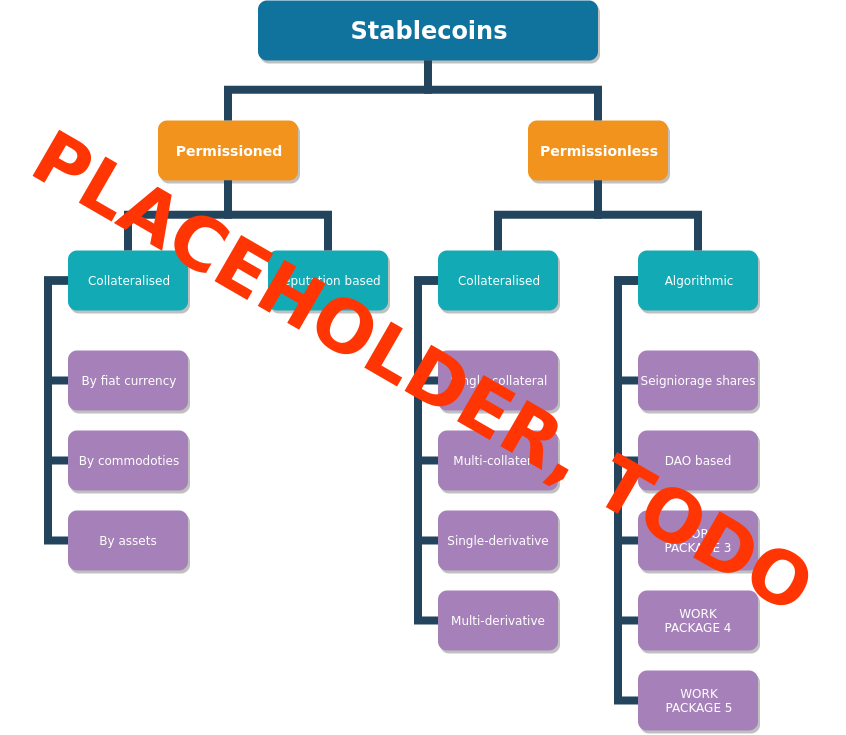
\includegraphics{img/intro.png}
\caption{Taxonomy of stablecoins \label{intro_label}}
\end{figure}

To manage market forces a diverse set of strategies have emerged, which
can be categorised in the categories visualised in \ref{intro_label}.
The easiest way to manage the price is through centralisation. This is
the permissioned category, these stablecoins are generally managed by an
organisation that keeps a tight leash on the coin and uses themselves as
a trusted third party similar to a central bank.

The permissionless category has as a primary goal to stay decentralised.
This comes with larger challenges, but also a greater potential to
deliver on the promise of a permissionless monetary system.

\begin{figure}[htbp]
\centering
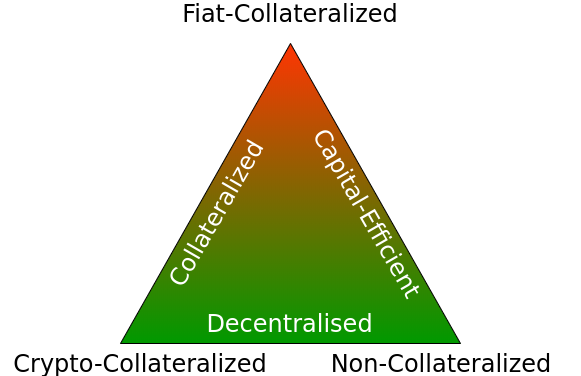
\includegraphics{img/Triangle.png}
\caption{Inherent trade-offs of stablecoins \label{triangle_label}}
\end{figure}

Within this survey we will explore the most common techniques to
stabilise cryptocurrencies, and show the inherent trade-offs between
decentralisation, collateralization, and capital efficiency as
illustrated in \ref{triangle_label}.

First, in chapter 2, we discuss the topic of the purpose of money, the
meaning of value and stability, and some currency pegs used in our
traditional monetary system. We then describe the simplest and most
successful stablecoins, namely the centralised coins in Chapter 3. In
Chapter 4 we go into the more complex topic of decentralised assets and
their methods for maintaining pegs to real world assets without a
central party guaranteeing the peg. We then go deeper into the theory in
Chapter 5 where we look at the research into the viability of
stablecoins. We then end with a discussion of the research on
stablecoins in Chapter 6 and a conclusion of the survey in Chapter 7.

\section{Background}\label{background}

{[}Bladwijzer - All above is somewhat done, all below is worked on{]}

Before we dive into the techniques for stabilisation, some definitions,
concepts and terms need to be established. In this section we review the
purpose and requirements of money. A model is described to explain the
forces acting upon the price of a currency. And some traditional
techniques for currency and asset stabilisation are reviewed. This will
give the necessary background to understand the different techniques
used by the different stablecoins.

\subsection{What is a good currency?}\label{what-is-a-good-currency}

In ``On the Origin of Money'' {[}1{]} Karl Menger describes how people
settle on a currency as a method of exchange. He describes that the
willingness of people to exchange their goods for a commodity depends:

\begin{enumerate}
\def\labelenumi{\arabic{enumi}.}
\tightlist
\item
  Upon their ability to trade it for goods
\item
  Upon the scarcity of the commodity
\item
  Upon the divisibility, durability and practicality of the commodity.
\item
  Upon the development of the market, and how others speculate.
\item
  Upon the limitations imposed politically and socially upon exchange,
  consumption and transfer from one period of time to another
\end{enumerate}

All these aspects must be managed in any successful currency. Points 2,
3 and possibly 5 are where cryptocurrencies have added value, through
their digital and decentralised natures. Points 1 and 4, the future
usefulness of the currency and it's market demand, are where
cryptocurrencies still fall short of traditional currencies. If
cryptocurrencies are going to replace traditional currencies, they have
to meet the last requirements of a good currency.

Stablecoins aim meet the last requirements, by adding guarantees about
the development of of the price in any market. This will in turn make
merchants more willing to accept the currency, thus providing the
ability to trade the currency for goods.

\subsection{What determines the price of an
asset?}\label{what-determines-the-price-of-an-asset}

The law of supply and demand model how the price of an asset in a market
is determined by the amount on offer versus the amount requested at any
given time. This model does a great job explaining and predicting price
changes following events that impact either. For the purpose of
controlling the price however, we need a model that gives us inputs that
we can affect. As both demand and supply are usually controlled by
independent actor in a market, we look at the quantity theory of money
instead.

In The Value of Money {[}2{]} Pigou describes the role of the money
supply in the Quantity theory of money and its relation to the price.
The quantity theory of money states:

\[ M \times V = p \times T \]

Where \(M\) is the total money supply, \(V\) is the velocity of
circulation, \(p\) is the price of good and services and \(T\) is the
total volume of transactions.

Note that \(p\) is the price of goods and services, and is thus the
inverse of the price of the currency. For easy of understanding we will
use an adapted version of the theory:

\[ M \times V \times P = T \]

Where \(P\) is the price of the currency.

The velocity of circulation \(V\) is a measure of how quickly money is
spent after receiving it. Together with the total money supply \(M\) it
makes up the supply side of the theory. If the total money supply goes
up, everything else being equal, the

This implies that the price of a currency can be controlled by
increasing and decreasing the money supply. Indeed this is a technique
also currently used by central to prevent deflation of their currencies.

In this survey we will see currencies vary both \(M\) and \(V\) as a
means to keep \(P\) at a stable level.

An certain configuration of these factors is required for a stable store
of value, and need to be controlled by some mechanism in order to
maintain a stable price of the commodity.

\subsection{Traditional means of stabilising a
currency}\label{traditional-means-of-stabilising-a-currency}

\subsection{Making a market}\label{making-a-market}

The easiest way to keep a currency stable is to simply have it derive
its value from a different asset that already has the desired stability.
This is called pegging.

The pegging of a token to an asset can be achieved by allowing investors
to trade the token for the asset at any time. Note that a this may
involve the trade of a secondary asset as intermediary store of value.

The first pegs were tracking the value of gold. Every unit of a currency
could be exchanged for a certain amount of gold. As described in ``The
Gold Standard'' {[}3{]} by Cooper, the US dollar has been pegged to Gold
for some of its years to maintain the confidence of the public.

The most common way to guarantee an exchange rate is to hold some form
of collateral. The most obvious collateral for the token, is the asset
it is pegged to, but this can also be another commodity that can be
traded for the asset at any time. Of course this requires some
guarantees or assumptions about the price stability of this commodity to
ensure that all outstanding tokens can be redeemed. If the amount of
collateral, or the value of the collateral, is such that less that 100\%
of tokens can be redeemed for the original asset, the token is
considered under-collateralized. This can have large ramifications to
investor trust, and might thus undermine the stability of the coin and
the viability of the network.

Any entity or system that facilitates the exchange of the token for the
collateral is called a market maker. In this survey two main categories
of market makers will make an appearance, centralised organisations and
decentralised systems.

\section{Stabilisation by
Centralisation}\label{stabilisation-by-centralisation}

With more control over the supply of a currency, the price stabilisation
of a currency is significantly simplified. Minting more in times of high
demand, though looked down upon, is a powerful way of controlling the
value of a currency and preventing runaway deflation. Conversely,
reducing the rate of minting slows down inflation of the currency.

Another way of stabilising a currency is to peg it to an already
existing currency or commodity. This method brings with it questions
about collateralization, transparency, risk, and the meaning of value.

In this section we explore the techniques employed by both central
reserve, and pegged stablecoins.

\subsection{The reserve bank
stablecoin}\label{the-reserve-bank-stablecoin}

Combining the proven success of central banks with the benefits of fast
payment systems {[}4{]}, organisations like JPMorgan {[}5{]} and the
Libra Association {[}6{]} aim to create a stable currency by using their
reputation as established financial institutions. So far, no coin has
managed to be stable off of its reputation alone, and whether this will
ever happen is yet to be seen.

\subsection{Pegged by currency
reserves}\label{pegged-by-currency-reserves}

Since stabilisation by reputation is often not good enough for investors
looking for a safe store of value, a stablecoin with stringer guarantees
about its future value is needed. The simplest way to do this is to
simply peg the cryptocurrency to another currency and guaranteeing a 1:1
exchange rate by holding enough collateral in order to make any investor
whole at any time in the future.

\begin{figure}[htbp]
\centering
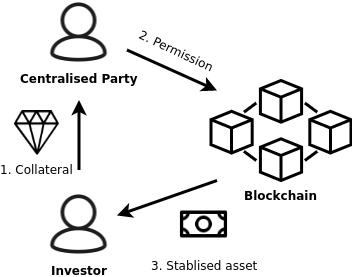
\includegraphics{img/Centralised_create.png}
\caption{Minting a pegged crypto-asset \label{cent_create_label}}
\end{figure}

Figure \ref{cent_create_label} describes the general way in which pegged
crypto assets are created. The centralised party in the image provides
some guarantee about the exchange rate. For this example we assume a peg
for 1 stabilised asset to always be worth 1 dollar. In this context, the
dollar is provided as collateral for the asset in the following way.

\begin{enumerate}
\def\labelenumi{\arabic{enumi}.}
\tightlist
\item
  1 dollar is transferred from the investor to the centralised party
  using traditional payment systems.
\item
  The centralised party mints 1 stabilised asset and transfers it to the
  investor
\item
  The investor is free to use the asset as they please
\end{enumerate}

\begin{figure}[htbp]
\centering
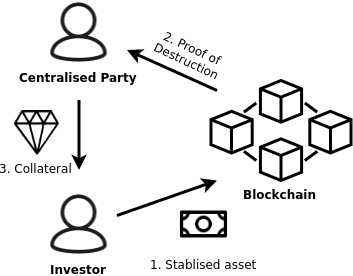
\includegraphics{img/Centralised_destroy.png}
\caption{Burning a pegged-crypto asset \label{cent_destoy_label}}
\end{figure}

Figure \ref{cent_destoy_label} illustrates the general way in which
pegged crypto assets can be traded back for the original asset.

\begin{enumerate}
\def\labelenumi{\arabic{enumi}.}
\setcounter{enumi}{-1}
\tightlist
\item
  Anyone can obtain the stabilised asset by trading for it on some
  market or by having one minted by the centralised party.
\item
  Any investor who holds a stabilised asset can send it to the
  blockchain to be burned.
\item
  Upon receiving a proof of destruction, the centralised party will send
  an equivalent amount of dollars back to the investor.
\item
  The investor is now out of their position.
\end{enumerate}

By guaranteeing that there is always a 1:1 exchange rate between the
collateral and the stabilised asset, the asset is pegged at a 1:1 ratio
even in external markets. This illustrated using the following two
scenarios.

When the stabilised asset trades for more than 1 dollar on the open
market, anyone can make an instant profit by minting more assets, and
immediately selling them on the open market. This process will continue
to increase the supply of the asset until the price is back down to 1
dollar.

Conversely, when the stabilised asset trades for less than 1 dollar on
the open market, anyone can make an instant profit by buying the coins
on the open market, and immediately burning them. This process will
continue to decrease the supply of the asset until the price is back up
to 1 dollar.

\subsubsection{Benefits of
Centralisation}\label{benefits-of-centralisation}

Like illustrated in figure \ref{triangle_label}, fiat-collateralized
pegs can not be maintained by a fully decentralised system. The limiting
factor is the fact that fiat-currencies need to be held by some party.

Some argue the price guarantees of pegging to a fiat-currency outweighs
the sacrifice of decentralisation. The success of currencies like Tether
{[}7{]}, Centres USDC {[}8{]}, PAXos {[}9{]}, and TrueUSD{[}10{]}
illustrate this with their combined market capitalization of 5 Billion
USD.

\subsubsection{Critiques of Centralisation and
solutions}\label{critiques-of-centralisation-and-solutions}

It goes without saying that having a centralised storage of anything
creates a central point of failure and control. Since trust in the
crypto space has long been based on what is verifiable, proving the
absence of fraud becomes a new challenge. To address the concerns of
coin holders the different stablecoin market makers provide different
guarantees with respect to the proper storage of collateral. Common ways
to improve investor confidence include:

\begin{enumerate}
\def\labelenumi{\arabic{enumi}.}
\tightlist
\item
  Regular audits providing proof of collateral (Tether {[}7{]}, USDC
  {[}8{]}, PAXos {[}9{]}, TrueUSD {[}10{]})
\item
  Multiple independent collateral trust accounts (TrueUSD
  {[}TrueUSD:whitepaper{]}, Stasis Euro {[}11{]})
\item
  Subjecting themselves to established regulations and providing FDIC-
  insurance. (PAXos {[}9{]})
\end{enumerate}

Through these means stablecoin organisations aim to counteract the lack
of transparency and the risk of under-collateralization.

\subsubsection{Expansions on fiat-currency
pegging}\label{expansions-on-fiat-currency-pegging}

Essentially, a centralised currency-pegged stablecoin is just a
tokenised fiat-currency. This concept can be expanded to more than just
traditional currencies. Using tokenisation and central storage it is
possible to peg the value of a crypto coin to anything that has value in
the real world. As such some stablecoins peg their value to the original
form of money: Gold. Today, stablecoins like PAX Gold {[}12{]} and
DigixDAO {[}13{]} hold gold in trust for their crypto holders. Though
the gold provides a strong guarantee that the stablecoin will hold its
value, the coins are still less stable than the Dollar as there is no
central agency stabilising gold.

Expanding even further on the concept of tokenised assets as
stablecoins, any collection of assets that is stable on average can
provide a stablecoin. Even though the US Dollar is seen as the most
stable currency world-wide, it is still dependent on the stability of
the United States economy. To address this stablecoins like Globcoin
{[}14{]} and x8currency {[}15{]} aim to create an asset that tracks
multiple currencies as well as gold. Thus creating a coin that is ``more
stable'' than the US Dollar. Whether these coins will ever have a
mainstream appeal is impossible to predict, but the theoretical value of
having a globally stable coin is hard to dispute.

\subsubsection{Overview of the largest
stablecoins}\label{overview-of-the-largest-stablecoins}

To provide a glimpse of the usage of the techniques described in this
subsection, Table \ref{TODO} describes the 8 central stablecoins with
the highest market capitalisation and some of their operational aspects:

\begin{longtable}[]{@{}lllllll@{}}
\toprule
\begin{minipage}[b]{0.14\columnwidth}\raggedright\strut
Stablecoin\strut
\end{minipage} & \begin{minipage}[b]{0.08\columnwidth}\raggedright\strut
Market Cap\strut
\end{minipage} & \begin{minipage}[b]{0.08\columnwidth}\raggedright\strut
Pegged asset\strut
\end{minipage} & \begin{minipage}[b]{0.10\columnwidth}\raggedright\strut
Escrow\strut
\end{minipage} & \begin{minipage}[b]{0.08\columnwidth}\raggedright\strut
FDIC-insurance\strut
\end{minipage} & \begin{minipage}[b]{0.04\columnwidth}\raggedright\strut
Launch\strut
\end{minipage} & \begin{minipage}[b]{0.30\columnwidth}\raggedright\strut
Notes\strut
\end{minipage}\tabularnewline
\midrule
\endhead
\begin{minipage}[t]{0.14\columnwidth}\raggedright\strut
Tether{[}7{]}\strut
\end{minipage} & \begin{minipage}[t]{0.08\columnwidth}\raggedright\strut
4 Trillion USD\strut
\end{minipage} & \begin{minipage}[t]{0.08\columnwidth}\raggedright\strut
USD\strut
\end{minipage} & \begin{minipage}[t]{0.10\columnwidth}\raggedright\strut
Single organisation\strut
\end{minipage} & \begin{minipage}[t]{0.08\columnwidth}\raggedright\strut
No\strut
\end{minipage} & \begin{minipage}[t]{0.04\columnwidth}\raggedright\strut
2014\strut
\end{minipage} & \begin{minipage}[t]{0.30\columnwidth}\raggedright\strut
Largest Stablecoin, 4th largest cryptocurrency\strut
\end{minipage}\tabularnewline
\begin{minipage}[t]{0.14\columnwidth}\raggedright\strut
USDC{[}8{]}\strut
\end{minipage} & \begin{minipage}[t]{0.08\columnwidth}\raggedright\strut
464 Million USD\strut
\end{minipage} & \begin{minipage}[t]{0.08\columnwidth}\raggedright\strut
USD\strut
\end{minipage} & \begin{minipage}[t]{0.10\columnwidth}\raggedright\strut
Single organisation\strut
\end{minipage} & \begin{minipage}[t]{0.08\columnwidth}\raggedright\strut
Some exchanges\strut
\end{minipage} & \begin{minipage}[t]{0.04\columnwidth}\raggedright\strut
2018\strut
\end{minipage} & \begin{minipage}[t]{0.30\columnwidth}\raggedright\strut
Created and owned by various crypto exchanges\strut
\end{minipage}\tabularnewline
\begin{minipage}[t]{0.14\columnwidth}\raggedright\strut
PAXos{[}9{]}\strut
\end{minipage} & \begin{minipage}[t]{0.08\columnwidth}\raggedright\strut
238 Million USD\strut
\end{minipage} & \begin{minipage}[t]{0.08\columnwidth}\raggedright\strut
USD\strut
\end{minipage} & \begin{minipage}[t]{0.10\columnwidth}\raggedright\strut
Single organisation\strut
\end{minipage} & \begin{minipage}[t]{0.08\columnwidth}\raggedright\strut
Yes\strut
\end{minipage} & \begin{minipage}[t]{0.04\columnwidth}\raggedright\strut
2018\strut
\end{minipage} & \begin{minipage}[t]{0.30\columnwidth}\raggedright\strut
Regulated by the New York State Department of Financial Services\strut
\end{minipage}\tabularnewline
\begin{minipage}[t]{0.14\columnwidth}\raggedright\strut
TrueUSD{[}10{]}\strut
\end{minipage} & \begin{minipage}[t]{0.08\columnwidth}\raggedright\strut
161 Million USD\strut
\end{minipage} & \begin{minipage}[t]{0.08\columnwidth}\raggedright\strut
USD\strut
\end{minipage} & \begin{minipage}[t]{0.10\columnwidth}\raggedright\strut
Multiple independent\strut
\end{minipage} & \begin{minipage}[t]{0.08\columnwidth}\raggedright\strut
Some escrows\strut
\end{minipage} & \begin{minipage}[t]{0.04\columnwidth}\raggedright\strut
2018\strut
\end{minipage} & \begin{minipage}[t]{0.30\columnwidth}\raggedright\strut
Distributes risk with multiple independent escrows\strut
\end{minipage}\tabularnewline
\begin{minipage}[t]{0.14\columnwidth}\raggedright\strut
Stasis{[}11{]}\strut
\end{minipage} & \begin{minipage}[t]{0.08\columnwidth}\raggedright\strut
35 Million USD\strut
\end{minipage} & \begin{minipage}[t]{0.08\columnwidth}\raggedright\strut
Euro\strut
\end{minipage} & \begin{minipage}[t]{0.10\columnwidth}\raggedright\strut
Multiple independent\strut
\end{minipage} & \begin{minipage}[t]{0.08\columnwidth}\raggedright\strut
No\strut
\end{minipage} & \begin{minipage}[t]{0.04\columnwidth}\raggedright\strut
2018\strut
\end{minipage} & \begin{minipage}[t]{0.30\columnwidth}\raggedright\strut
Largest Euro Stablecoin\strut
\end{minipage}\tabularnewline
\begin{minipage}[t]{0.14\columnwidth}\raggedright\strut
BUSD{[}9{]}\strut
\end{minipage} & \begin{minipage}[t]{0.08\columnwidth}\raggedright\strut
18 Million USD\strut
\end{minipage} & \begin{minipage}[t]{0.08\columnwidth}\raggedright\strut
USD\strut
\end{minipage} & \begin{minipage}[t]{0.10\columnwidth}\raggedright\strut
Single organisation\strut
\end{minipage} & \begin{minipage}[t]{0.08\columnwidth}\raggedright\strut
Yes\strut
\end{minipage} & \begin{minipage}[t]{0.04\columnwidth}\raggedright\strut
2019\strut
\end{minipage} & \begin{minipage}[t]{0.30\columnwidth}\raggedright\strut
Issued by PAXos for the Binance exchange\strut
\end{minipage}\tabularnewline
\begin{minipage}[t]{0.14\columnwidth}\raggedright\strut
USDK\strut
\end{minipage} & \begin{minipage}[t]{0.08\columnwidth}\raggedright\strut
28 Million USD\strut
\end{minipage} & \begin{minipage}[t]{0.08\columnwidth}\raggedright\strut
USD\strut
\end{minipage} & \begin{minipage}[t]{0.10\columnwidth}\raggedright\strut
Single organisation\strut
\end{minipage} & \begin{minipage}[t]{0.08\columnwidth}\raggedright\strut
No\strut
\end{minipage} & \begin{minipage}[t]{0.04\columnwidth}\raggedright\strut
2019\strut
\end{minipage} & \begin{minipage}[t]{0.30\columnwidth}\raggedright\strut
Owned and operated by the oklink exchange\strut
\end{minipage}\tabularnewline
\begin{minipage}[t]{0.14\columnwidth}\raggedright\strut
PAX Gold{[}12{]}\strut
\end{minipage} & \begin{minipage}[t]{0.08\columnwidth}\raggedright\strut
12 Million USD\strut
\end{minipage} & \begin{minipage}[t]{0.08\columnwidth}\raggedright\strut
Gold (1 ounce)\strut
\end{minipage} & \begin{minipage}[t]{0.10\columnwidth}\raggedright\strut
Single organisation\strut
\end{minipage} & \begin{minipage}[t]{0.08\columnwidth}\raggedright\strut
No\strut
\end{minipage} & \begin{minipage}[t]{0.04\columnwidth}\raggedright\strut
2019\strut
\end{minipage} & \begin{minipage}[t]{0.30\columnwidth}\raggedright\strut
Gold held in custody by PAXos Trust Company\strut
\end{minipage}\tabularnewline
\bottomrule
\end{longtable}

Some interesting observations can be made from the table.

\begin{enumerate}
\def\labelenumi{\arabic{enumi}.}
\tightlist
\item
  The PAXos company operates 3 of the top 8 stablecoins.
\item
  3 of the top 8 stablecoins are operated by exchanges including the
  second largest stablecoin USDC.
\item
  Gold based stablecoins still make up a small portion of the market
  with PAX Gold being the largest with a market cap of 12 million.
\end{enumerate}

\section{Stabilised while
Decentralised}\label{stabilised-while-decentralised}

Though many centralised stablecoins are becoming more diversified in
their collateralization, the organisations that run them remain a
central point of failure. The risk of collateral depletion by market
maker failure is always prevalent and though some stablecoins store
their collateral with bankruptcy remote companies, this just moves the
risk to a different central entity.

To protect investors from the failure of any central entity and even the
failure of the financial system as a whole, new stablecoins have emerged
that remain price-stable in a decentralised manner. These coins come in
two main categories:

\begin{enumerate}
\def\labelenumi{\arabic{enumi}.}
\tightlist
\item
  Crypto-Collateralized Stablecoins
\item
  Algorithmic Stablecoins
\end{enumerate}

This section explains the mechanisms that keep these coins stable,
provides a comparison of their advantages and disadvantages, and a
general overview of the largest decentralised stablecoins on the market
right now in each category.

\subsection{Crypto-Collateralized
Stablecoins}\label{crypto-collateralized-stablecoins}

The success of the centralised stablecoins shows that the backing of a
stablecoin with 100\% collateral is a reliable way to keep a currency
price stable.

The main problem with backing a decentralised stablecoin with some type
of collateral is that there needs to be a mechanism of exchange between
the stablecoin and the collateral. When the collateral is fiat-currency
or some real world asset, there must always be a central party that
holds the collateral and facilitates the mechanism of exchange.

Crypto-collateralized coins build on the idea that a holder of a
stablecoin can always get their share of the collateral back, but in a
fully automated and decentralised manner.

Crypto-collateral coins allow the exchange of the pegged currency such
that even the organisation that created the stablecoin has no power over
the collateral. Initially it may seem like we need a collateral with the
following requirements:

\begin{enumerate}
\def\labelenumi{\arabic{enumi}.}
\tightlist
\item
  Stable - to stabilise the stablecoin
\item
  Decentralised - to avoid central control
\item
  Fully programmable - to automate the collateral exchange mechanism
\end{enumerate}

The problem here is quite obvious, we are looking for precisely the
thing we are trying to create, a decentralised stablecoin. In order to
solve this, crypto-collateralized stablecoins choose drop the 3rd
requirement and use decentralised but unstable cryptocurrencies as
collateral. The way this can still lead to a stable currency is as
follows:

Instead of guaranteeing the direct exchange of the stablecoin for the
pegged currency, say 1 token for 1 dollar, the system aims to guarantee
that an investor can exchange 1 token for 1 dollars worth of the
collateral at any time. This leaves a problem, what if, because of the
volatility of the collateral, the market value of the collateral drops
such that there is no longer enough collateral to back all outstanding
stablecoins. This could lead investors to scramble to get their share of
the collateral out before its gone, rapidly undermining the price of the
stablecoin.

The solution to this is overcollateralization. In order to guarantee
that there is always enough collateral in the system for every investor
to be made whole, the creation of any stablecoin has to be paired with
the deposit of \textbf{more} than 100\% collateral.

This leads to one final question, what investor looking to hedge against
the price stability of cryptocurrencies would lock up their crypto in
order to get a token that has lower value than the underlying
collateral. They are now neither hedged against the drop in value of
their collateral, nor do they have any extra utility with their new
token as the collateral was equally decentralised and programmable.

The solution to this is found in the concept of a swap. A financial swap
is a derivative contract where two parties swap some properties of some
underlying assets. In the case of our stablecoin, one party, lets call
them the investor, offloads the risk associated with the price
instability of the collateral to our second party, lets call them the
speculator.

\begin{figure}[htbp]
\centering
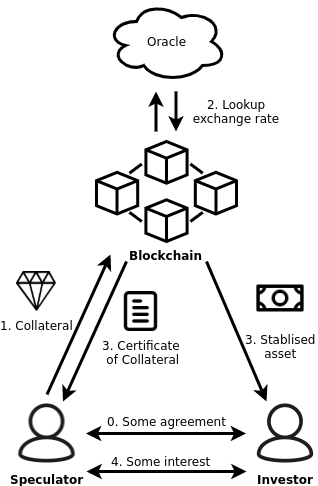
\includegraphics{img/CDP_create.png}
\caption{Stablecoin minting through debt creation
\label{cdp_destroy_label}}
\end{figure}

Figure \ref{cdp_destroy_label} describes the process of minting a
decentralised stablecoin that uses the swap mechanic:

\begin{enumerate}
\def\labelenumi{\arabic{enumi}.}
\setcounter{enumi}{-1}
\tightlist
\item
  Some agreement is reached between the investor and the speculator.
  This might happen on an individual basis, but sometimes the terms of
  the agreement are pre-defined by parameters of the network.
\item
  Some crypto, lets say Ether, is sent as collateral to a
  smart-contract. Some of this, usually 100\%, might come from the
  investor, white the speculator provides the rest of the collateral,
  lets say 50\%, for the stablecoin to remain overcollateralized by some
  ratio, in this case 150\%.
\item
  A smart-contract checks the price of the Ether in terms of the pegged
  currency, lets say dollars. Mechanisms for the decentralised lookup of
  Ether prices vary between systems. We explore these differences later
  in this section.
\item
  The stablecoin is minted and issued to the investor, while the
  speculator gets some proof of deposit for their collateral. Lets call
  this the debt-contract.
\item
  Some interest might be payed from the investor to the speculator or
  vise versa.
\end{enumerate}

The investor might pay interest to the speculator as a reward for
providing the capital for overcollateralization and taking on the risk
of the collateral dropping in value while the stablecoin is in
circulation. On the other hand, the speculator might pay the investor as
a reward for providing extra capital for the speculator to leverage
their bet on Ether. The direction of interest depends on the design of
the stablecoin and sometimes the market conditions.

While the stablecoin is in circulation the speculator is responsible for
maintaining the collateral of debt-contract. Should the value of Ether
drop, they must deposit more Ether to the smart contract, or risk
getting margin called.

A margin call is the automatic closing of a debt contract. A margin call
happens when the value of the collateral drops below the minimum
collateral requirement of the system. In the case of our example this
means there is not enough Ether in the debt-contract to cover 150\% of
the outstanding stablecoins of the contract. A margin call opens the
debt-position to be closed by anyone, and incentivises this by providing
a reward for whoever closes it.

The closing of a contract is the burning of the stablecoin and the
recovery of the underlying collateral. The process for this is
illustrated in figure \label{cdp_destroy_label} and includes the
following steps:

\begin{enumerate}
\def\labelenumi{\arabic{enumi}.}
\setcounter{enumi}{-1}
\tightlist
\item
  Some agreement is reached between an investor willing to sell a
  stablecoin, and a someone willing to close out a debt-contract. This
  agreement could come be in the form of a speculator simply buying the
  coins from an investor at market rate, an investor acting on a margin
  call, or by some other matching mechanism between stablecoin and
  debt-contract.
\item
  The stablecoin is sent to a smart-contract, which burns the coin.
\item
  The oracle is consulted for the current price level of Ether in
  dollars.
\item
  The collateral is provided back to the speculator and investor at some
  defined ratio. Ususally 100\% of the stablecoin value goes to the
  investor while the remaining 50\% or more goes back to the speculator.
\item
  Some settlement may be done, this could be the payment of interest
  between the two parties or some fee to the blockchain.
\end{enumerate}

\begin{figure}[htbp]
\centering
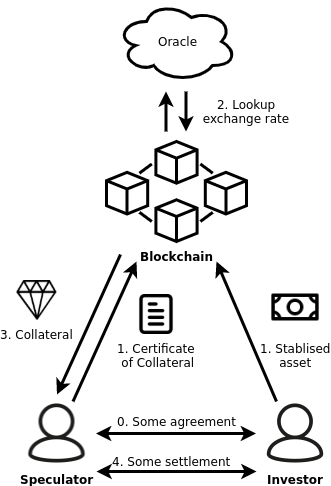
\includegraphics{img/CDP_destroy.png}
\caption{Stablecoin burning through debt-position closage
\label{cdp_destroy_label}}
\end{figure}

As an extra line of defence against the falling of the collateral value
or some attack against the system, crypto-collateralized stablecoins
often have a mechanism for global settlement implemented. In the case of
a global settlement event, the underlying collateral gets returned to
the investors without any conditions. All debt contracts will be locked,
allowing all holders of the stablecoin to trade in their tokens for 1
dollars worth of collateral. After a period of time, the contracts will
be released and return all collateral left back the the speculators.

The triggers for a global settlement differ per stablecoin, but
mechanisms include: global collateralization under a minimum ratio, high
price instability, a decision by holders of some governance token.

\subsubsection{Governance}\label{governance}

In addition to triggering global settlement in the case of some black
swan event, decisions need to be made about the network in general.
Examples of this can be parameter tweaking like the collateralization
ratio or network fees, as well as network upgrades. For this reason most
decentralised stablecoins are part of a Distributed Autonomous
Organisation (DAO). Shares in the DAO, or governance tokens, allow the
holders some say over the inner workings of the network, as well as some
claim of the profits of the network. This ties the value of the tokens
to the to the performance of the network, which in turn incentivises the
holders of the governance tokens to remain invested in the network and
to vote for parameters and mechanisms that improve the utility and
stability of the stablecoin.

\subsubsection{Minimum Collateralization
Ratio}\label{minimum-collateralization-ratio}

The minimum collateral required varies between systems. It is the
responsibility of the speculator to maintain a collateralization ratio
above the minimum requirement, or they get margin called.

The collateralization requirement depends on the volatility of the
collateral used. Since the margin call of a contract takes time to find
an investor someone willing to close it, there needs to be a buffer for
the price of the collateral to fall even further. This buffer is the gap
between the minimum ratio and 100\%.

This means that network doesn't lose any collateral as long as the
collateral doesn't drop to \(1/c\) within the time it takes to margin
call a contract. Where \(c\) is the minimum collateralization ratio.

\subsubsection{Mechanism for speculator to investor match
making}\label{mechanism-for-speculator-to-investor-match-making}

Stablecoins that utilise these derivative contracts are usually built
with a system that aligns the incentives of the stablecoins within some
structure. Variations in these systems leads to differences in features
like:

\begin{itemize}
\tightlist
\item
  the direction of interest payments,
\item
  the matching of investor to speculator,
\item
  the amount of collateral put up by each party,
\item
  the mechanism of a margin call or forced-settlement.
\end{itemize}

To explain the variation between the systems we use some examples. We
show how defences in the purpose of the system leads to differences in
the features, and how the price keeps stabilising.

\paragraph{Reserve bank speculator
model}\label{reserve-bank-speculator-model}

In the first type of system the speculators collectively act like a
reserve bank.

The creation and destruction of stablecoins are controlled by the
speculator. Anyone can create a debt-contract, deposit collateral and
mint stablecoin tokens as long as they remain properly
overcollateralized. The contract can also be closed at any time by
depositing an equal amount of stablecoins to get the same collateral
back.

It is important to know that, in this system, the amount of stablecoins
created is determined by the price, in say dollars, of the collateral at
the time of minting. This leads to the following incentive structure:

If the market value of the token is higher that 1 dollar a speculator is
incentivised to deposit more collateral and mint more tokens. These
token can then be sold on the market. Increasing the supply, thus
dropping the price back to one dollar. The benefit of the speculator
here is that they were able to create a debt contract at a favorable
rate. If, when they pay back the tokens, the market value of the token
is lower than when they sold the coins, they will make a profit.

If the market value of the token is lower than a dollar, any speculator
with an open contract can buy the tokens at a discount and close their
contract out at a profit given that they bought sold the tokens at a
higher price. This leads to fewer coins on the market, thus increasing
the value back up to a dollar.

This creates a ``soft peg'' as there is no guarantee for the speculator
that when they mint and a coin they will be able to buy it back again at
a lower price. This can lead to the market price of the token rising to
a different price level, and the peg can stabilise at a price level that
is higher or lower than any collateral held.

The price level of the token is thus determined by what the market
believes it is worth. There is some indication however, that the coin
will not drop below 1 dollar, since that is the value that is returned
to investors in the case of margin calls or a global settlement
scenario.

In this scenario, the speculator takes on a certain amount of risk
speculating on the value of the collateral and the price of the token.
Initially it seems like the speculator gets their value from speculation
only. They can, for example, sell their tokens on the market for more of
the collateral thus leveraging their speculation on the collateral by
some factor.

Usually, the designer intended way for the speculator to make a profit
is by peer to peer lending. Instead of selling the tokens on the market,
the speculator can lend out the tokens to makes some extra dividends
while speculating on the collateral. In this way, the speculator acts as
the reserve bank increasing the supply of the token by lending out more.

Irregardless of how the speculator chooses to use their tokens, anyone
investor buying them has a some guarantee that they will be worth at
least a dollar in the future, thus creating an asset that is more stable
than the underlying collateral.

The complete risk acceptance and decision making of the speculator
allows for a number of expansions on the already explained concepts.
First, since the success of the network is dependent on everyone being
properly collateralized on average, and this in turn is dependent on the
market value of the collateral, it makes sense to diversify the
collateral. Thus, a multi-collateral system, which improves guarantees
for token holders can be created, where the speculators have a choice in
what collateral they want to stake. This protects the system against a
price crash in one collateral category, as speculators are incentivised
to exchange the collateral that is dropping in value for more
price-stable collateral.

\paragraph{Speculation market model}\label{speculation-market-model}

In this model the stablecoin can still be bought by the investor to
offload risk to a speculator on some market. On the other side of the
coin, the speculator still puts up extra collateral to back the coin in
order to speculate on the underlying assets and provide collateral in
case of a price dip.

The first differences between this model and the reserve bank model is
that the mechanism to match investor to speculator, hereafter called the
``internal market'', is done through margin trading. This means that the
internal market is effectively an exchange where speculators and
investors put up offers to be matched with each other.

The model relies on the fact that the investor, at any time, can redeem
the stablecoin for 1 dollars worth of collateral. This way the price
should always be around 1 dollar.

When a speculator puts up an offer, it acts like a proposal to the
investor. The offer describes the amount of collateral that the investor
should pay into the debt position. The investor knows that they have
some guarantee to redeem it for 1 dollar of collateral at any point
later. This fact provide a lower bound on the value of the coin as coins
sold below a dollar will immediately be bought up and redeemed. This
creates a price for the investor of 1 dollar plus some premium. This
premium acts as an incentive for the speculator to put up the extra
collateral and is variable based on the market.

After two orders get matched on the internal market, the investor
provides the agreed upon amount of collateral, and the speculator puts
up the rest of the collateral required to meet the minimum ratio and
maintains this throughout the lifetime of the contract.

The generated stablecoin is given to the investor and is fully fungible
as they can be redeemed for 1 dollar at any time regardless of how much
collateral the first investor put up. The coin can now be traded just
like any other currency on some external market.

Interest in this is payed from the speculator to the investor, as the
investor allows the speculator to use their collateral to speculate on.

When finally a stablecoin holder wants to close out their side of the
contract and redeem their dollar of collateral, they make another order
on the internal market. They will then get matched with a speculator
wishing to close out their contract.

The investor gets 1 dollar of collateral from the contract of the
speculator, and the speculator gets the rest. At this point the
speculator will take their earnings or losses as they will have get more
collateral than they put in if the price of the collateral has gone up,
and they will lose collateral if the price of the collateral has gone
down.

In order to make sure there are always enough speculators willing to
settle a stablecoin, this model can employ some ways of forcing
speculators to match the settlement. The first way is a maximum lifetime
for speculator contracts. This forces speculators to close out their
contract within a set time, say 30 days. This guarantees that any
investor can redeem their coin within this time as the full outstanding
amount of stablecoins in the system have to be bought back every 30 day.
The second way is to simply close out the speculators contract that has
the lowest collateral ratio. This has the benefit that investors get
their money back quicker than the first option. This also incentives the
speculator keep a high collateralization ratio.

This system, though similar, is fundamentally different from the reserve
bank model in that the speculation is meant act like a prediction market
while the stablecoin aspect is secondary. It also has the issue that
there needs to be some exchange mechanism to match orders.

This system differs from the reserve bank model in the fact that the
guarantee for the investor generated after 2 people create a coin
together. The first and last investor are always interacting through the
internal market, which causes the investor to be more that just someone
looking for a safe position. As the investor buys the coin at some
``premium'' they are betting that the price on the market when they want
to sell accounts for this premium.

However, when buying a coin on the open market this stablecoin is only
subject to the change in the premium and not the volatility of the coin.

The feasibility of this mechanism is yet to fully prove itself in
reality, though some steps have been made. The BitShares exchange was
the first to use this mechanism and originally implemented a 30 day
limit for speculator contracts, thus guaranteeing a maximum liquidation
delay of 30 days. This was stable for a while but eventually lead to a
distrust in the ``guarantee'' that the coin was redeemable, as you
essentially have to freeze your asset for 30 days to get your money
back. This lead to the value of BitUSD dropping, which lead in turn lead
to people ``shorting'' BitUSD by taking worse and worse prices for the
stablecoin, as they expected to be able to close their contracts while
the price of BitUSD was even lower. This created a negative feedback
loop where the dropping price of BitUSD acturally provided an incentive
to create more BitUSD.

As a result, the BitShares holders voted for global settlement to avoid
the further loss of stability. Eventually the stablecoin was relaunched
with the 30 day limit removed and a 24 hour guarantee built in that
matches the settlement order with the lowest collateralized contract.
The price has not made it back to one dollar and remains relatively
volatile.

Other BitShares stablecoins like BitCNY also use this mechanism and are
stable, likely because of a larger, thus more resilient, market.

\paragraph{Debt-pool Tracker service}\label{debt-pool-tracker-service}

The final matchmaking system is very similar to the reserve bank system,
but abstracts away from the concept of having a single stablecoin, and
just aims to track the prices of many different assets.

The system tracks the total debt of a speculator, rather than the
specific stablecoin assets. This means that, just like in the reserve
bank model, a speculator can put up any amount of collateral and issue
``debt'' based on some collateralization ratio. This means that the
speculator is again the party that provides the stability, and absorbs
any price shocks to the collateral.

As an investor the story changes. Any holder of a stablecoin can
directly exchange it for a different stablecoin of equal value, at any
time, using only the blockchain. Like before, the investor buys the
stablecoin on the market. Lets say they buy a stablecoin that tracks the
dollar. The blockchain allows them to exchange it for a stablecoin that
tracks the euro at some exchange rat between the dollar and the euro.

Since no money was created, the total value in the system did not change
and thus no interaction with the underlying collateral was needed. This
allow the system to create synthetic assets that track any underlying
assets, including currencies, stocks, other cryptos, and even the
inverse of these.

When a speculator wants to leave the system, they simply have to buy
back some assets worth what they originally created before they get
their collateral back.

In this system interest is periodically payed from all investors to all
speculators as incentive for the speculators to collateralize the
system.

This system can provide a whole ecosystem for tracking real world assets
and allows easy movement between them.

\subsubsection{Overview}\label{overview}

As can be seen in \ref{TODO} There are a few large players in the crypto
collateralized stablecoin scene.

\begin{longtable}[]{@{}lllllll@{}}
\toprule
\begin{minipage}[b]{0.12\columnwidth}\raggedright\strut
Stablecoin (System)\strut
\end{minipage} & \begin{minipage}[b]{0.04\columnwidth}\raggedright\strut
Peg\strut
\end{minipage} & \begin{minipage}[b]{0.10\columnwidth}\raggedright\strut
Collateral\strut
\end{minipage} & \begin{minipage}[b]{0.06\columnwidth}\raggedright\strut
Min. col.\strut
\end{minipage} & \begin{minipage}[b]{0.16\columnwidth}\raggedright\strut
Matchmaking\strut
\end{minipage} & \begin{minipage}[b]{0.20\columnwidth}\raggedright\strut
Interest paid\strut
\end{minipage} & \begin{minipage}[b]{0.12\columnwidth}\raggedright\strut
Governance (token)\strut
\end{minipage}\tabularnewline
\midrule
\endhead
\begin{minipage}[t]{0.12\columnwidth}\raggedright\strut
DAI (MakerDAO)\strut
\end{minipage} & \begin{minipage}[t]{0.04\columnwidth}\raggedright\strut
USD\strut
\end{minipage} & \begin{minipage}[t]{0.10\columnwidth}\raggedright\strut
Ether (and more)\strut
\end{minipage} & \begin{minipage}[t]{0.06\columnwidth}\raggedright\strut
150\%\strut
\end{minipage} & \begin{minipage}[t]{0.16\columnwidth}\raggedright\strut
Reserve bank speculator model\strut
\end{minipage} & \begin{minipage}[t]{0.20\columnwidth}\raggedright\strut
To Speculator (external)\strut
\end{minipage} & \begin{minipage}[t]{0.12\columnwidth}\raggedright\strut
DAO (MKR)\strut
\end{minipage}\tabularnewline
\begin{minipage}[t]{0.12\columnwidth}\raggedright\strut
BitAssets (BitShares)\strut
\end{minipage} & \begin{minipage}[t]{0.04\columnwidth}\raggedright\strut
Multi\strut
\end{minipage} & \begin{minipage}[t]{0.10\columnwidth}\raggedright\strut
BTS\strut
\end{minipage} & \begin{minipage}[t]{0.06\columnwidth}\raggedright\strut
300\%\strut
\end{minipage} & \begin{minipage}[t]{0.16\columnwidth}\raggedright\strut
Margin Trading\strut
\end{minipage} & \begin{minipage}[t]{0.20\columnwidth}\raggedright\strut
Variable premium, once to speculator\strut
\end{minipage} & \begin{minipage}[t]{0.12\columnwidth}\raggedright\strut
DAO (BTS)\strut
\end{minipage}\tabularnewline
\begin{minipage}[t]{0.12\columnwidth}\raggedright\strut
Synths (Synthetix)\strut
\end{minipage} & \begin{minipage}[t]{0.04\columnwidth}\raggedright\strut
Multi\strut
\end{minipage} & \begin{minipage}[t]{0.10\columnwidth}\raggedright\strut
SNX\strut
\end{minipage} & \begin{minipage}[t]{0.06\columnwidth}\raggedright\strut
750\%\strut
\end{minipage} & \begin{minipage}[t]{0.16\columnwidth}\raggedright\strut
Debt-Pool Tracker\strut
\end{minipage} & \begin{minipage}[t]{0.20\columnwidth}\raggedright\strut
Global interest calculation\strut
\end{minipage} & \begin{minipage}[t]{0.12\columnwidth}\raggedright\strut
Centralsed, DAO soon\strut
\end{minipage}\tabularnewline
\begin{minipage}[t]{0.12\columnwidth}\raggedright\strut
USDQ (QDAO)\strut
\end{minipage} & \begin{minipage}[t]{0.04\columnwidth}\raggedright\strut
USD\strut
\end{minipage} & \begin{minipage}[t]{0.10\columnwidth}\raggedright\strut
Bitcoin\strut
\end{minipage} & \begin{minipage}[t]{0.06\columnwidth}\raggedright\strut
200\%\strut
\end{minipage} & \begin{minipage}[t]{0.16\columnwidth}\raggedright\strut
Reserve bank speculator model\strut
\end{minipage} & \begin{minipage}[t]{0.20\columnwidth}\raggedright\strut
To Speculator (external)\strut
\end{minipage} & \begin{minipage}[t]{0.12\columnwidth}\raggedright\strut
DAO (QDAO)\strut
\end{minipage}\tabularnewline
\bottomrule
\end{longtable}

MakerDAO is currently the largest most trusted system. They now allow
for multiple different types of collateral, including Ether, BAT, REP
and X0. They allow the community to vote using their (MKR) token. On
which assets will be added for collateral.

BitShares is the system with one of the oldest working stablecoin,
BitCNY, active since september 2014. BitShares is a decentralised
exchange that allows users to speculate on a number of different
BitAssets, including BitUSD, BitEUR, and BitBTC.

Synthetix describes itself as a ``synthetic asset platform'' and
provides a number of stablecoins that track multiple real world
currencies and assets. They allow direct conversion from one to another
using the debt-pool tracker system where speculators are collateralizing
the system at a minimum of 750\%. The Synthetix platform started of
centralised and is still a work in progress but is making major steps
towards decentralisation. They offer many tracking assets like: sEUR,
sUSD, sBTC, sETH. They also offer inverted assets to bet against some
assets like: iBTC, and iETH. Currently they also support commodities
like sXAU which tracks the Philadelphia Gold and Silver Index, and they
plan to add trackers for various company stocks.

\subsection{Non-collateralized
Stablecoins}\label{non-collateralized-stablecoins}

Crypto collateralized stablecoins are dependent on the overall stability
of their collateral currency. If the price of the collateral drops fast
enough in relation to the pegged currency, many of these stablecoins
would lose their exchange guarantee, and therefore lose investor
confidence. Though these risks can be reduced in various ways, the
general stabilisation of a currency without the reliance on collateral
is a sought after feature that could improve significantly stablecoins.

Some stablecoins, rather than offloading risk to speculators, aim to
reduce volatility by controlling the demand and supply of currencies in
other ways. In this section we describe the securities model for
expanding and contracting the money supply, as well as some more
theoretical techniques and currency parameters for reducing volatility.

\subsubsection{Securities model}\label{securities-model}

The stabilisation of currencies is much older than cryptocurrencies. So
to see how cryptocurrencies can be stabilised, some have taken
inspiration from the way central banks stabilise traditional currencies.
Specifically open market operations employed by central banks and the
federal reserve.

When the fed wants to increase the money supply in times of deflation,
they often buy government securities thus getting money out into the
hands of the public. When they then want to decrease the money supply,
they will sell the securities thus getting the money out of the system.

The securities stablecoin model utilises this concept. In times of
inflation when the currency is undervalued, the blockchain will start
selling bonds. These bonds lock up a buyers coins for a period of time,
and will pay them back, including some interest, after a certain time.
Since some of the money is now temporally out of circulation, the
currency left on the market will go up in value.

In times of deflation when the currency in overvalued, bonds can be
discouraged or disabled. Outstanding bonds can also be payed back
prematurely in order to increase the money supply. When all bonds have
released and deflation is still a problem, more money can be printed and
distributed in some way until there the price is back down to the
desired level.

Variables that can be tweaked to maintain the desired price level are:

\begin{itemize}
\tightlist
\item
  The interest payed over the bond - higher encourages purchase
\item
  The lifetime of the bond - this is how long the money is out of
  circulation
\end{itemize}

These techniques have the potential to stabilise a currency without any
collateral being needed. However, the choice of when the money supply
should be expanded or retracted still needs to be made in a
decentralised way. Consequently this is where the largest differences
between the existing stablecoins lie.

\paragraph{Self stabilisation
mechanisms}\label{self-stabilisation-mechanisms}

By tweaking bond lifetime and interest rates a currency can be
stabilised. However there still needs to be some decentralised mechanism
that triggers changes to these parameters. Usually one of two self
stabilising mechanisms is used:

\begin{itemize}
\tightlist
\item
  Share voting based parameter setting
\item
  An Oracle based price feedback mechanism
\end{itemize}

Voting based parameter setting works how one would expect. The holders
of a token, in some cases the stablecoin itself but usually a governance
token, vote periodically on the stabilisation parameters of the network.

Within the oracle based system, the blockchain will activate an
``expansion phase'' in a time where the price of the coin is above the
target, and a ``contraction phase'' when the price is below the target.
The bond yield can be static or scale with how far the price is from the
target, thus rewarding larger risk takers.

Note that even oracle based stablecoins are usually DAO's that vote on
the function that maps price target mismatch to bond parameters.

\subsubsection{Overview of real world non-collateralized
stabilising}\label{overview-of-real-world-non-collateralized-stabilising}

\begin{longtable}[]{@{}llllll@{}}
\toprule
\begin{minipage}[b]{0.27\columnwidth}\raggedright\strut
Stablecoin (System)\strut
\end{minipage} & \begin{minipage}[b]{0.06\columnwidth}\raggedright\strut
Target\strut
\end{minipage} & \begin{minipage}[b]{0.19\columnwidth}\raggedright\strut
Stabilisation Mechanism\strut
\end{minipage} & \begin{minipage}[b]{0.09\columnwidth}\raggedright\strut
Duration\strut
\end{minipage} & \begin{minipage}[b]{0.08\columnwidth}\raggedright\strut
Interest\strut
\end{minipage} & \begin{minipage}[b]{0.15\columnwidth}\raggedright\strut
Governance (token)\strut
\end{minipage}\tabularnewline
\midrule
\endhead
\begin{minipage}[t]{0.27\columnwidth}\raggedright\strut
Nubits\strut
\end{minipage} & \begin{minipage}[t]{0.06\columnwidth}\raggedright\strut
USD\strut
\end{minipage} & \begin{minipage}[t]{0.19\columnwidth}\raggedright\strut
Voting\strut
\end{minipage} & \begin{minipage}[t]{0.09\columnwidth}\raggedright\strut
Voted\strut
\end{minipage} & \begin{minipage}[t]{0.08\columnwidth}\raggedright\strut
Voted\strut
\end{minipage} & \begin{minipage}[t]{0.15\columnwidth}\raggedright\strut
DAO (NuShares)\strut
\end{minipage}\tabularnewline
\begin{minipage}[t]{0.27\columnwidth}\raggedright\strut
BitBay {[}16{]}\strut
\end{minipage} & \begin{minipage}[t]{0.06\columnwidth}\raggedright\strut
None\strut
\end{minipage} & \begin{minipage}[t]{0.19\columnwidth}\raggedright\strut
Voting\strut
\end{minipage} & \begin{minipage}[t]{0.09\columnwidth}\raggedright\strut
Unlimited\strut
\end{minipage} & \begin{minipage}[t]{0.08\columnwidth}\raggedright\strut
None\strut
\end{minipage} & \begin{minipage}[t]{0.15\columnwidth}\raggedright\strut
DAO (BitBay)\strut
\end{minipage}\tabularnewline
\begin{minipage}[t]{0.27\columnwidth}\raggedright\strut
Anchor{[}17{]}\strut
\end{minipage} & \begin{minipage}[t]{0.06\columnwidth}\raggedright\strut
\strut
\end{minipage}\tabularnewline
\begin{minipage}[t]{0.27\columnwidth}\raggedright\strut
Basis{[}18{]}\strut
\end{minipage} & \begin{minipage}[t]{0.06\columnwidth}\raggedright\strut
USD\strut
\end{minipage} & \begin{minipage}[t]{0.19\columnwidth}\raggedright\strut
Oracle\strut
\end{minipage} & \begin{minipage}[t]{0.09\columnwidth}\raggedright\strut
5 years\strut
\end{minipage} & \begin{minipage}[t]{0.08\columnwidth}\raggedright\strut
Voted\strut
\end{minipage} & \begin{minipage}[t]{0.15\columnwidth}\raggedright\strut
DAO\strut
\end{minipage}\tabularnewline
\begin{minipage}[t]{0.27\columnwidth}\raggedright\strut
Ampleforth {[}19{]}\strut
\end{minipage} & \begin{minipage}[t]{0.06\columnwidth}\raggedright\strut
\strut
\end{minipage}\tabularnewline
\bottomrule
\end{longtable}

The first stablecoin to be stable for a year was NuBits{[}20{]}. NuBits
stabilised by using a bond mechanism as well as voted in ``guardians''
who would get newly printed NuBits and would in turn provide liquidity
to the market. These guardians would sell and buy the NuBits on the
market at the price determined by the peg. In a way this turns the
guardians into holders of collateral.

NuBits lost their peg twice and successfully recovered once in 2016, but
after the ``Christmas crash'' of late 2017-2018 investors massively
bought the stablecoin as presumably it was safe compared to the rest of
the crashing crypto market because of its peg to the dollar. This grew
the market cap of NuBits by 1500\% over a few months while the guardians
mostly held collateral in bitcoin. When then the crypto market started
to recover, many sold their NuBits putting large pressure on the
guardians who were now forced to buy NuBits for fewer bitcoins than they
bought then for during the crash. This under-collateralized NuBits to a
point where the guardians ran out of collateral, the currency lost its
price guarantee, and the peg could no longer be maintained.

NuBits provides an example of the main flaw of the securities model, it
requires trust in the mechanism, which lacks when it is needed most: in
a down market.

\subsection{Oracles}\label{oracles}

All stablecoins that peg to a fiat currency need some information about
the price of that currency at any point in time. So far we have referred
to Oracles as a source of this. In reality, this is a non-trivial
problem and it is solved in a couple different ways.

The simplest solution is having a centralised source, this does create a
central point of control and thus a central point of failure. When there
is a central party that facilitates the exchange, this is not a problem.

Efforts have been made to decentralise the oracles as well. When every
other aspect of the network is decentralised, a decentralised oracle
will provide more security, which in turn boosts investor trust as this
removes the central point of failure.

One way to decentralise the network is to have all nodes in the network
vote on the value of the input. Here a proof of stake system can be used
that punishes bad inputs to the system. If there are multiple different
values given, the median can be taken.

Some decentralised currencies have a DAO token or similar that is tied
to the health of the network. Since the value of the DAO token is
dependent on the health of the network, holders of this token are
incentivised to act honestly. In addition, some punishment for bad
behaviour can be added in the form of proof of stake to aid in
determining the correct price.

This mechanism also more specifically applicable, just determining
precise price levels. Some stablecoins do not track the price, but have
token holders vote whether the price is too high or too low, and based
on that will trigger either ``inflationary'', or ``deflationary''
periods {[}16{]}.

This concept can also generalised even further. A long desired goal is
to get real world information onto the blockchain in general. Solutions
have emerged {[}21{]} that aim to solve this problem by creating a
general infrastructure of nodes that access real world data and record
this data onto the blockchain. To incentivise honesty of nodes, they
stake an amount of network tokens that can be taken from them if the
rest of the network disagrees with their votes. In addition node
reputation van be tracked on-chain in order to allow users to choose the
most trustworthy nodes.

\subsection{General techniques for adding stability to any
currency}\label{general-techniques-for-adding-stability-to-any-currency}

Collateralized stablecoins by definition are pegged currencies. They
rely on other currencies to provide their stability. Without the
stability of the US dollar or other, none of these currencies would
work. When it comes to inherent stability of blockchain currencies, a
number of academic papers are available. Following is a survey of
techniques to reduce the volatility of any decentralised blockchain
based currency.

\subsubsection{Changing proof of work parameters to dampen demand
shocks}\label{changing-proof-of-work-parameters-to-dampen-demand-shocks}

Taking the quantity theory of money as a given, the price of a currency
depends on the total supply, velocity of circulation, and the total
amount transacted. These things are often set by the parameters of a
blockchain network.

In the case of Bitcoin, the total supply is set, and slowly increased at
a set rate without reacting to supply and demand. However, there is a
link between the price levels and mining efforts {[}22{]}. If the price
of bitcoin drops below a certain level, the mining reward will no longer
outweigh the electricity costs. This miner response to the markets gives
a natural input that somewhat tracks the price.

The block speed, and therefore the rate of supply of new coins, increase
as the price increases. Therefore, if the mining difficulty stays the
same, the currency will naturally respond to, and dampen, demand shocks
{[}22{]}.

Additionally, if the block speed is changed, the transaction throughput
changes proportionally. This has the extra benefit of changing the
velocity of money, which dampens the demand shock even further.

It is important to keep in mind that there are both upper and lower
technical limits to the block speed. Set it too low and the transaction
throughput suffers. Conversely if the block speed is too high forks are
more likely, which undermines the security of the network.

\subsubsection{Allowing for inflation}\label{allowing-for-inflation}

This method of controlling price levels has some implications {[}22{]}
on long term price. In bitcoin, long term inflation is curbed by
periodically halving the block reward. If these changes were used, this
system would unnecessarily lower the mining incentives for miners, thus
leading to a lower block rate.

One solution is to no longer halve the block rewards, thus turning
Bitcoin into an inflationary currency. This is very controversial and
has large economic implications who's details go beyond the scope of
this survey.

As it is not possible to remove currency from the market, some rate of
coin depreciation might be desirable to allow for absorption of future
demand shocks {[}23{]}. A coin depreciation rate can be applied by
gradually increasing the mining rewards over time.

\subsubsection{Open mining using Proof of Sequential
Work}\label{open-mining-using-proof-of-sequential-work}

If block speed should remain constant, a different way to build a more
stable currency is to build a secondary token. This token would use
Proofs of Sequential work (PoSW) {[}24{]} to generate currency at a
fixed rate. This allows anyone to mine a coin by putting in some work.
This leads more mining when the price is high and less when it is low.

PoSW has the benefit of scaling better into the future as the sequential
speed of processors improve at a much slower rate than parallel speeds.

\section{Discussions of Stablecoins}\label{discussions-of-stablecoins}

Stablecoins are an even younger development in the young field of
cryptocurrencies. As such it isn't yet clear how the future of
stablecoins will look. In addition to the currently existing stablecoins
and proposed stablecoin concepts, research is being done into the
general viability and security of stablecoins. This section discusses
the viability of stablecoins and aims to answer more general question
about their future and usefulness.

\subsection{Centralised Stablecoins}\label{centralised-stablecoins}

Centralised stablecoins have so far found their usecase as a stable way
to store your crypto away from volatility and bear markets. When looking
to the future, much literature is available exploring where stablecoins
can become useful.

When looking at ways cryptocurrencies can improve the current financial
system centralised stablecoins can be seen as a midway solution
{[}25{]}. It marries the stability and legal security of central trusted
organisations, with the benefits of fast, programmable and more
transparent payment systems {[}4{]} {[}26{]}. This leads to a system
that relies less trust in large banks.

\subsection{Crypto Collateralized
Stablecoins}\label{crypto-collateralized-stablecoins-1}

Decentralised currencies are more aspirational. Where Bitcoin provided a
completely trust less currency. Decentralised currencies aim to do the
same, but with guarantees about price stability. Though this is much
more difficult to get working securely {[}27{]}, the benefit of these
coins to society might be much greater than that of any centralised
currency.

Separate from the issue of price stable currency, many decentralised
stablecoins have shown decentralised alternatives to mechanisms like
contracts for difference {[}TODO cite something{]}. Even if these
mechanisms don't end up working for stablecoins in the long term, they
still mark an important step in the world of Decentralised Finance
(DeFi).

\subsection{Related Work}\label{related-work}

\subsubsection{Surveying the stablecoin
space}\label{surveying-the-stablecoin-space}

In ``The State of Stablecoins''{[}28{]} the ``blockchain team'' present
an empirical study of 57 live and pre-launch stablecoins showing
adoption, trading volume and market cap. They describe a taxonomy where
they differentiate between ``traditional'' collateralized, crypto
collateralized and algorithmic. They describe many pros and cons of
these types of coins. The survey is very extensive and describes all 57
currencies in terms of their investors, tech, legal structure and
collateral format.

\subsubsection{Speculating on the future of
stablecoins}\label{speculating-on-the-future-of-stablecoins}

In {[}4{]} Darrel Duffie describes the use of stablecoins for banks
aiming to digitise both inter-organisation value transfer and
governments wanting to implement a digital currency with the utility
benefits of cryptocurrencies and the stability of fiat.

In ``Stablecoins in Cryptoeconomics. From Initial Coin Offerings (ICOs)
to Central Bank Digital Currencies''{[}26{]} Erba discusses the
stablecoins in the context of the law in both the united states and
Europe. Erba argues for crypto-currencies ``fully backed by Central Bank
reserves''

In {[}25{]} Koning describes the requirements and considerations for a
stable currency controlled by a central bank. Koning describes the
monetary policy and choices that comes along with implementing a digital
currency on a large scale.

\subsubsection{Critiques of common techniques for cryptocurrency
stabilisation}\label{critiques-of-common-techniques-for-cryptocurrency-stabilisation}

Chohan discusses the difficulties in maintaining a properly
collateralized peg in ``Are Stable Coins Stable?''{[}29{]}. Chohan
describes how maintaining a true 1:1 peg leads to funding and
scalability issues.

In {[}27{]} Klages-Mundt et al. look at the existing stablecoins through
a critical lens and describe some ways in which the currency pegs can be
broken. Klages-Mundt build a generalised model of decentralised
crypto-collateralized stablecoins. It describes possible attacks on
these systems where the pegged currency is bid up so an extent where
collateral starts to get margin-called creating a run-away feedback
loop.

\section{Conclusion}\label{conclusion}

There is a lot happening in the stablecoin and DeFi space right now.
Stablecoins are being tested in a trial by fire in the real-world as we
speak. Through this organisations such as MakerDAO and Synthetix are
developing completely systems that promise to either revolutionise the
world by taking Decentralised Finance to the next level, or they will
spectacularly go up in a ball of fire. Only time will tell.

\section*{References}\label{references}
\addcontentsline{toc}{section}{References}

\hypertarget{refs}{}
\hypertarget{ref-On_the_Origin_of_Money}{}
{[}1{]} K. Menger, ``On the Origin of Money,'' \emph{The Economic
Journal}, vol. 2, no. 6, pp. 239--255, Jun. 1892.

\hypertarget{ref-Value_of_Money}{}
{[}2{]} A. C. Pigou, ``The Value of Money,'' \emph{The Quarterly Journal
of Economics}, vol. 32, no. 1, pp. 38--65, Nov. 1917.

\hypertarget{ref-The_Gold_Standard}{}
{[}3{]} R. N. Cooper, R. Dornbusch, and R. E. Hall, ``The gold standard:
Historical facts and future prospects,'' \emph{Brookings Papers on
Economic Activity}, vol. 1982, no. 1, pp. 1--56, 1982.

\hypertarget{ref-DuffieDigital_and_Fast_Payment_Systems}{}
{[}4{]} D. Duffie, ``DuffieDigital and fast payment systems,'' MONTHH
YEARR.

\hypertarget{ref-JPMorgan_Coin:whitepaper}{}
{[}5{]} JPMorgan Chase \& Co., ``J.P.Morgan coin announcement.''
\url{https://www.jpmorgan.com/global/news/digital-coin-payments},
MONTHH-YEARR.

\hypertarget{ref-Libra:whitepaper}{}
{[}6{]} ``Libra whitepaper.''
\url{https://libra.org/en-US/white-paper/}, MONTHH-YEARR.

\hypertarget{ref-Tether:whitepaper}{}
{[}7{]} Tether International Limited, ``Tether whitepaper.''
\url{https://tether.to/wp-content/uploads/2016/06/TetherWhitePaper.pdf},
MONTHH-YEARR.

\hypertarget{ref-Centre:whitepaper}{}
{[}8{]} CENTRE Consortium, ``Centre whitepaper.''
\url{https://www.centre.io/pdfs/centre-whitepaper.pdf}, MONTHH-YEARR.

\hypertarget{ref-PAXos:whitepaper}{}
{[}9{]} Charles Cascarilla, ``PAXos whitepaper.''
\url{https://account.paxos.com/whitepaper.pdf}, MONTHH-YEARR.

\hypertarget{ref-TrueUSD:whitepaper}{}
{[}10{]} LLC TrueCoin, ``Trust token.''
\url{https://www.trusttoken.com/trueusd}, MONTHH-YEARR.

\hypertarget{ref-Stasis:whitepaper}{}
{[}11{]} STASIS Foundation, ``Stasis whitepaper.''
\url{https://stasis.net/}, MONTHH-YEARR.

\hypertarget{ref-PAXGold:whitepaper}{}
{[}12{]} Charles Cascarilla, ``PAX gold whitepaper.''
\url{https://www.paxos.com/paxgold/}, Sept-2019.

\hypertarget{ref-DigixDAO:whitepaper}{}
{[}13{]} Anthony C. Eufemio, ``DigixDAO whitepaper.''
\url{https://digix.global/whitepaper.pdf}, MONTHH-YEARR.

\hypertarget{ref-globcoin:whitepaper}{}
{[}14{]} Reserve Currency Solutions, ``Globcoin whitepaper.''
\url{https://globcoin.io/assets/pdf/whitepaper-Globcoin-v3.1.0.pdf},
MONTHH-YEARR.

\hypertarget{ref-x8currency:whitepaper}{}
{[}15{]} X8 AG, ``X8currency whitepaper.''
\url{https://x8currency.com/wp-content/uploads/X8-Project-TGE-Whitepaper.pdf},
MONTHH-YEARR.

\hypertarget{ref-BitBay:whitepaper}{}
{[}16{]} David Zimbeck, ``BitBay whitepaper.''
\url{https://bitbay.market/downloads/whitepapers/bitbay-dynamic-peg.pdf},
MONTHH-YEARR.

\hypertarget{ref-Anchor:whitepaper}{}
{[}17{]} Anchor AG, ``Anchor whitepaper.''
\url{https://theanchor.io/whitepaper/}, MONTHH-YEARR.

\hypertarget{ref-Basis:whitepaper}{}
{[}18{]} Josh Chen Nader Al-Naji and Lawrence Diao, ``Basis
whitepaper.'' \url{https://www.basis.io/basis_whitepaper_en.pdf},
MONTHH-YEARR.

\hypertarget{ref-Ampleforth:whitepaper}{}
{[}19{]} Brandon Iles Evan Kuo and Manny Rincon Cruz, ``Ampleforth.''
\url{https://www.ampleforth.org/paper/}, MONTHH-YEARR.

\hypertarget{ref-Nubits:whitepaper}{}
{[}20{]} Jordan Lee, ``Nubits whitepaper.''
\url{https://nubits.com/whitepaper}, MONTHH-YEARR.

\hypertarget{ref-Chainlink:whitepaper}{}
{[}21{]} Steve Ellis, ``Chainlink whitepaper.''
\url{https://link.smartcontract.com/whitepaper}, MONTHH-YEARR.

\hypertarget{ref-How_to_make_a_digital_currency_on_a_blockchain_stable}{}
{[}22{]} K. Saito and M. Iwamura, ``How to make a digital currency on a
blockchain stable,'' \emph{Future Generation Computer Systems}, vol.
100, 2019.

\hypertarget{ref-CanWeStabilize}{}
{[}23{]} M. Iwamura, Y. Kitamura, T. Matsumoto, and K. Saito, ``Can we
stabilize the price of a cryptocurrency?: Understanding the design of
bitcoin and its potential to compete with central bank money.''

\hypertarget{ref-Elasticoin_Low-Volatility_PoSW}{}
{[}24{]} R. B. Yuhao Dong, ``Elasticoin: Low-volatility posw,'' MONTHH
YEARR.

\hypertarget{ref-Fedcoin}{}
{[}25{]} J. P. Koning, ``Fedcoin\_Central\_Bank\_R3.pdf,''
\url{https://www.r3.com/reports/fedcoin-a-central-bank-issued-cryptocurrency/},
MONTHH YEARR.

\hypertarget{ref-Stablecoins_in_Cryptoeconomics}{}
{[}26{]} M. Dell'Erba, ``Stablecoins in cryptoeconomics. from initial
coin offerings to central bank digital currencies (cbdcs),'' MONTHH
YEARR.

\hypertarget{ref-In_stability_for_the_Blockchain}{}
{[}27{]} A. M. Ariah Klages-Mundt, ``(In)stability for the blockchain:
Deleveraging spirals and stablecoin attacks,'' MONTHH YEARR.

\hypertarget{ref-THE_STATE_OF_STABLECOINS}{}
{[}28{]} T. B. Team, ``The state of stablecoins,'' MONTHH YEARR.

\hypertarget{ref-Are_Stable_Coins_Stable}{}
{[}29{]} U. W. Chohan, ``Are stable coins stable?'' MONTHH YEARR.

\end{document}

